% Options for packages loaded elsewhere
\PassOptionsToPackage{unicode}{hyperref}
\PassOptionsToPackage{hyphens}{url}
%
\documentclass[
]{article}
\usepackage{amsmath,amssymb}
\usepackage{iftex}
\ifPDFTeX
  \usepackage[T1]{fontenc}
  \usepackage[utf8]{inputenc}
  \usepackage{textcomp} % provide euro and other symbols
\else % if luatex or xetex
  \usepackage{unicode-math} % this also loads fontspec
  \defaultfontfeatures{Scale=MatchLowercase}
  \defaultfontfeatures[\rmfamily]{Ligatures=TeX,Scale=1}
\fi
\usepackage{lmodern}
\ifPDFTeX\else
  % xetex/luatex font selection
\fi
% Use upquote if available, for straight quotes in verbatim environments
\IfFileExists{upquote.sty}{\usepackage{upquote}}{}
\IfFileExists{microtype.sty}{% use microtype if available
  \usepackage[]{microtype}
  \UseMicrotypeSet[protrusion]{basicmath} % disable protrusion for tt fonts
}{}
\makeatletter
\@ifundefined{KOMAClassName}{% if non-KOMA class
  \IfFileExists{parskip.sty}{%
    \usepackage{parskip}
  }{% else
    \setlength{\parindent}{0pt}
    \setlength{\parskip}{6pt plus 2pt minus 1pt}}
}{% if KOMA class
  \KOMAoptions{parskip=half}}
\makeatother
\usepackage{xcolor}
\usepackage[margin=1in]{geometry}
\usepackage{longtable,booktabs,array}
\usepackage{calc} % for calculating minipage widths
% Correct order of tables after \paragraph or \subparagraph
\usepackage{etoolbox}
\makeatletter
\patchcmd\longtable{\par}{\if@noskipsec\mbox{}\fi\par}{}{}
\makeatother
% Allow footnotes in longtable head/foot
\IfFileExists{footnotehyper.sty}{\usepackage{footnotehyper}}{\usepackage{footnote}}
\makesavenoteenv{longtable}
\usepackage{graphicx}
\makeatletter
\def\maxwidth{\ifdim\Gin@nat@width>\linewidth\linewidth\else\Gin@nat@width\fi}
\def\maxheight{\ifdim\Gin@nat@height>\textheight\textheight\else\Gin@nat@height\fi}
\makeatother
% Scale images if necessary, so that they will not overflow the page
% margins by default, and it is still possible to overwrite the defaults
% using explicit options in \includegraphics[width, height, ...]{}
\setkeys{Gin}{width=\maxwidth,height=\maxheight,keepaspectratio}
% Set default figure placement to htbp
\makeatletter
\def\fps@figure{htbp}
\makeatother
\usepackage{soul}
\setlength{\emergencystretch}{3em} % prevent overfull lines
\providecommand{\tightlist}{%
  \setlength{\itemsep}{0pt}\setlength{\parskip}{0pt}}
\setcounter{secnumdepth}{-\maxdimen} % remove section numbering
\ifLuaTeX
  \usepackage{selnolig}  % disable illegal ligatures
\fi
\IfFileExists{bookmark.sty}{\usepackage{bookmark}}{\usepackage{hyperref}}
\IfFileExists{xurl.sty}{\usepackage{xurl}}{} % add URL line breaks if available
\urlstyle{same}
\hypersetup{
  pdftitle={EL PRESUPUESTO EN LOS AYUNTAMIENTOS},
  pdfauthor={Tomàs Ferrandis Moscardó},
  hidelinks,
  pdfcreator={LaTeX via pandoc}}

\title{EL PRESUPUESTO EN LOS AYUNTAMIENTOS}
\author{Tomàs Ferrandis Moscardó}
\date{2022-12-15}

\begin{document}
\maketitle

{
\setcounter{tocdepth}{2}
\tableofcontents
}
\hypertarget{introducciuxf3n}{%
\section{1 INTRODUCCIÓN}\label{introducciuxf3n}}

En el presente trabajo podemos diferenciar claramente dos bloques
temáticos. Un primer bloque empezará con el estudio de las fuentes de
financiación de los ayuntamientos de España centrándose en los
principales ingresos. A partir de los datos extraídos, podremos ver la
dependencia del presupuesto municipal con los presupuestos del resto de
administraciones (Estado, Diputaciones Provinciales y Comunidades
autónomas) así como la capacidad de recaudación propia de las Entidades
locales. Todo ello nos aportará una visión concreta y clara de la
estructura de los presupuestos públicos y la relación de dependencia
entre las diferentes administraciones, así como la dependencia entre
ingresos y gastos de cada una ellas y de todas en conjunto.

Para poder ilustrar la aportación de las autonomías y Diputaciones
Provinciaes en la financiación de los entes municipales hemos escogido
el caso de los municipios valencianos y el Fondo de Cooperación
Municipal de esta comunidad. No obstante, haremos alguna reflexión sobre
los diferentes criterios existentes en otras autonomías.

A partir de este punto estaremos en disposición de analizar brevemente
los distintos modelos de financiación municipal del mundo occidental y
exponer sus características básicas.

La segunda parte o bloque temático será una ampliación de los conceptos
que definen y caracterizan al presupuesto. Sin repetir las definiciones
y argumentaciones ya estudiadas, nos centraremos en las particularidades
de nuestro caso, el presupuesto municipal. Así identificaremos para cada
fase a los órganos responsables, los principios que la rigen y los
procesos que la definen en base la legislación estatal y autonómica.

A lo largo del tema, tras identificar cómo se materializan los distintos
principios económicos y políticos vistos en la asignatura, estudiaremos
dos cambios legislativos relacionados. Uno, específico de la
Administración Local que garantiza la aprobación del presupuesto
municipal en casos extremos de bloqueo por parte del pleno y el segundo,
general a todo el Sector Público relacionado con el control de la deuda
y el equilibrio presupuestario.

Concluiremos nuestro trabajo con las conclusiones sobre las dos
evoluciones históricas. La que permitió el desarrollo de más servicios
para los vecinos y, la aún en vigor, más echando ando del freno
economicista.

\hypertarget{el-presupuesto-general-en-los-ayuntamientos}{%
\section{2 EL PRESUPUESTO GENERAL EN LOS
AYUNTAMIENTOS}\label{el-presupuesto-general-en-los-ayuntamientos}}

En este apartado vamos a tratar de esclarecer las fórmulas que el Estado
usa para asignar parte del gasto del Presupuesto General a las entidades
locales y las Comunidades autónomas y, como éstas, a su vez, implementan
algún fondo especial para mejorar las arcas municipales bajo distintos
criterios políticos.

Dada la enorme complejidad en la financiación de las administraciones,
nuestro propósito es dar una pinceladas sobre el tema centrándonos en
los ayuntamientos al ser las entidades que ocuparían un nivel inferior y
están más afectadas por la subsidiariedad de las otras administraciones.

Como hemos comentado, las autonomías (como las Diputaciones
provinciales, forales o cabildos) pueden establecer, en aras de su
autonomía, sistemas distintos de ayudas para ayuntamientos o
agrupaciones de éstos, por lo que será necesario centrarse en alguna
autonomía y provincia. En nuestro caso hemos elegido la provincia de
Valencia.

En este tema se verá, por tanto, no solo la relación entre ingresos de
la recaudación y los gastos previstos sino también la relación entre
capítulos de gastos de la administración superior y los capítulos de
ingresos de la administración que recibe.

\hypertarget{financiaciuxf3n-local}{%
\section{3. FINANCIACIÓN LOCAL}\label{financiaciuxf3n-local}}

De forma detallada podemos indicar como recursos de los Ayuntamientos
los siguientes:

\begin{itemize}
\item
  Los tributos propios que son impuestos, tasas y contribuciones
  especiales.
\item
  Las participaciones en los tributos del Estado y de las comunidades
  autónomas.
\item
  Las subvenciones.
\item
  Operaciones de crédito.
\item
  Del patrimonio y demás de derecho privado.
\item
  Los percibidos en concepto de precios públicos.
\item
  Otros: precios públicos y otras prestaciones de derecho público,
  multas.
\end{itemize}

No obstante, como ya hemos avanzado, nos centraremos solo en tres
fuentes de ingresos: los tributos propios (especialmente el Impuesto
sobre Bienes Inmuebles), las participaciones del Estado y la
participación de las Comunidades Autónomas.

De las tres aportaciones debemos destacar por su importancia
cuantitativa, en primer lugar, los impuestos (concretamente el Impuesto
sobre Bienes Inmuebles, IBI) y, en segundo lugar, la aportación del
Estado. La tercera aportación, la participación autonómica, aunque tras
implantarse, ha ido creciendo, la estudiaremos por ser un rasgo
definitorio de algunos modelos de financiación local de los países
occidentales como ya hemos avanzado en la introducción. Además de su
interés político puesto debemos reseñar que su implantación generalizada
se realizó a partir de las penúltimas modificaciones estatutarias.

\hypertarget{tributos-propios}{%
\subsection{TRIBUTOS PROPIOS}\label{tributos-propios}}

\hypertarget{regulaciuxf3n}{%
\subsubsection{REGULACIÓN}\label{regulaciuxf3n}}

Atendiendo a los principios constitucionales, la legislación Estatal
determina que las Entidades Locales disponen de autonomía en materia
tributaria mediante la aprobación de dos instrumentos legales: las
\emph{Ordenanzas fiscales reguladoras de tributos} y las
\emph{Ordenanzas generales de gestión, recaudación e inspección}.

Las primeras, ordenanzas fiscales son las normas que regulan los
tributos municipales. Cada tributo requiere de una para determinar el
concepto, como se calcula y quien debe pagar además de posibles
bonificaciones o exenciones. Las segundas son la base reglamentario que
establece el procedimiento de cobro.

La aprobación o modificación de todas las ordenanzas corresponde al
pleno de la corporación.

\hypertarget{delegaciuxf3n-de-la-gestiuxf3n-tributaria}{%
\subsubsection{DELEGACIÓN DE LA GESTIÓN
TRIBUTARIA}\label{delegaciuxf3n-de-la-gestiuxf3n-tributaria}}

La gestión tributaria de los ayuntamientos puede delegarse en organismos
supramunicipales mediante acuerdo plenario. Es el caso de gran parte de
los pequeños y medianos municipios de la provincia de València que
delegan el cobro de todos o casi todos los tributos en la Diputación de
Valencia. Ésta, en contraprestación al servicio, cobra a los
Ayuntamientos una tasa calculada en base a la recaudación y, a su vez,
regulada en sus propias ordenanzas.

Otro ejemplo de externalización se da en los consorcios de servicios
como son el tratamiento de residuos o abastecimiento de agua potable,
dónde son estas mismas entidades supramunicipales las que emiten
directamente los recibos al contribuyente.

\hypertarget{cargas-sobre-usuarios-y-autonomuxeda-local}{%
\subsubsection{CARGAS SOBRE USUARIOS Y AUTONOMÍA
LOCAL}\label{cargas-sobre-usuarios-y-autonomuxeda-local}}

Pese a que las entidades locales tienen como función fundamental la
prestación de servicios, la incidencia de las tasas y precios públicos
cobrados en el total de los ingresos recaudados es prácticamente
testimonial.

\emph{Debate sobre las tasas y precios actualizados.}

A la hora de abordar la suficiencia financiera de los ayuntamientos
españoles, hay autores que, lo primero que ponen sobre la mesa, es la
necesidad de revisar estas cargas; entendiendo que la financiación de
los servicios debe ir a cargo de los beneficiados. Defendiendo que sea
una obligación para todos.

Pero la realidad es que el mundo local es reacio a esta imposición ``se
manifiesta de forma rotunda por la amplitud legal de los presupuestos de
hecho y de la cuantificación de las tasas: el ente local no solo
decidirá si establece o no la exacción de una concreta tasa, sino que
también determinará, con un amplio margen de actuación, su
cuantificación'' (Aragonés: 2011). Una visión donde se asume el
principio de autonomía local como de forma absoluta y que contrasta con
la de quienes ven en este tema una decisión de gran importancia política
además de ideológica.

\emph{Coste efectivo de los servicios.}

En la actualidad, la \emph{Ley 27/2013, de 27 de diciembre, de
racionalización y sostenibilidad de la Administración Local} establece
la obligación para todas las entidades locales de calcular el coste
efectivo de los servicios a partir de los datos del último ejercicio con
instrucciones precisas en cuanto a la fórmula.

\hypertarget{la-aportaciuxf3n-del-estado}{%
\subsection{LA APORTACIÓN DEL
ESTADO}\label{la-aportaciuxf3n-del-estado}}

Tras el Impuesto sobre Bienes Inmuebles Urbano (IBIU), este ingreso es
la segunda fuente de financiación en los municipios españoles.
Analizamos brevemente los dos sistemas de aportación a los municipios
por parte del Estado, sin entrar en las peculiaridades de los municipios
turísticos y su compensación extra. Existen dos regímenes, el general
para la mayoría de los municipios y el de cesion de tributos para
municipios con una población superior a 75.000 habitantes o capitales de
provincias o autonomía.

\hypertarget{en-municipios-de-menos-de-75.000-habitantes.}{%
\subsubsection{EN MUNICIPIOS DE MENOS DE 75.000
HABITANTES.}\label{en-municipios-de-menos-de-75.000-habitantes.}}

\textbf{Participación por variables en los tributos del Estado ( PTE )}

La Participación en los Tributos del Estado, en adelante PTE, es el
importe que destina el Estado a los municipios de menos de 75.000
habitante y que además no son capital de provincia o autonomía. Se trata
de una fracción de lo que recauda el Estado de los principales
impuestos, una vez ha hecho la cesión a las Comunidades Autónomas, es
decir los Ingresos Tributarios del Estado (en adelante ITE).

RECAUDACIÓN = IngresosTributariosEstado + Cesión CA + Participación
EntidadLocal

Los impuestos afectados son:

\begin{itemize}
\tightlist
\item
  IRPF
\item
  IVA
\item
  Impuestos especiales: Hidrocarburos, tabaco, cerveza, alcohol y
  productos Intermedios
\end{itemize}

CA: Comunidad Autónoma

EL: Entidad Local

\textbf{APORTACIÓN A LAS AUTONOMÍAS Y LOS AYUNTAMIENTOS. AÑO 2021}

\emph{Tabla 1. Aportación del Estado a partir de la información del
MHFP. (elaboración propia )}

\begin{longtable}[]{@{}
  >{\raggedright\arraybackslash}p{(\columnwidth - 8\tabcolsep) * \real{0.2000}}
  >{\raggedleft\arraybackslash}p{(\columnwidth - 8\tabcolsep) * \real{0.2000}}
  >{\raggedleft\arraybackslash}p{(\columnwidth - 8\tabcolsep) * \real{0.2000}}
  >{\raggedleft\arraybackslash}p{(\columnwidth - 8\tabcolsep) * \real{0.2000}}
  >{\raggedleft\arraybackslash}p{(\columnwidth - 8\tabcolsep) * \real{0.2000}}@{}}
\toprule\noalign{}
\begin{minipage}[b]{\linewidth}\raggedright
INGRESOS TRIBUTARIOS DEL ESTADO
\end{minipage} & \begin{minipage}[b]{\linewidth}\raggedleft
TOTAL
\end{minipage} & \begin{minipage}[b]{\linewidth}\raggedleft
PARTICIPACIÓN
\end{minipage} & \begin{minipage}[b]{\linewidth}\raggedleft
Adm.territoriales
\end{minipage} & \begin{minipage}[b]{\linewidth}\raggedleft
ITE
\end{minipage} \\
\midrule\noalign{}
\endhead
\bottomrule\noalign{}
\endlastfoot
\emph{Millones de euros} & & \emph{CA} & \emph{CL} & \\
IRPF & 94.545 & 49.470 & 1.083 & 43.993 \\
\textbf{CAPÍTULO I. IMPUESTOS DIRECTOS} & & & & \\
Impuesto sobre el Valor Añadido & 72.498 & 35.411 & 774 & 36.313 \\
IMPUESTOS ESPECIALES (1) & & & & \\
Alcohol y Bebidas Derivadas & 673 & 409 & 8 & 255 \\
Cerveza & 312 & 182 & 4 & 126 \\
Productos Intermedios & 22 & 12 & 0 & 10 \\
Hidrocarburos & 11.492 & 7.581 & 119 & 3.792 \\
Labores del Tabaco & 6.115 & 3.830 & 71 & 2.214 \\
Carbón & 29 & & & 29 \\
Electricidad & 1.086 & 1.399 & & 313 \\
Impuesto sobre Gases Fluorados & 65 & & & \\
Impuesto sobre Tráfico Exterior & 1.955 & & & \\
Imp. sobre las Primas de seguros & 2.052 & & & \\
Imp. sobre Transacciones Financieras & 296 & & & \\
Impuesto sobre Servicios Digitales & 166 & & & \\
Impuesto sobre Actividades del juego & 44 & & & \\
Otros Ingresos & 8 & & & \\
\textbf{CAPÍTULO II. IMPUESTOS INDIRECTOS} & & & & \\
Tasa & 784 & & & \\
Otros Ingresos & 1.205 & & & \\
\textbf{CAPÍTULO III. TASAS Y OTORS INGRESOS} & 1.989 & & & \\
\textbf{Total Ingresos Tributarios} & \textbf{260.800} & & & \\
\end{longtable}

\textbf{CÁLCULO DE LA PARTICIPACIÓN de TRIBUTOS del ESTADO}

Para el cálculo del valor de la PTE ( Participación de Tributos del
Estado ) tenemos:

\begin{enumerate}
\def\labelenumi{\alph{enumi}.}
\item
  Valor de base. El importe transferido en el año 2004.
\item
  Variación del ITE del último año liquidado ( años -2 ) respecto a

  \begin{enumerate}
  \def\labelenumii{\arabic{enumii}.}
  \setcounter{enumii}{2003}
  \tightlist
  \item
  \end{enumerate}
\end{enumerate}

Cálculo para el 2021:

\begin{itemize}
\item
  PTE 2004: 2.888.359.105,16
\item
  Índice ITE: 2019/2004: 1,4797
\end{itemize}

Como conclusiones podríamos extraer las dos consecuencias directas más
importantes:

\begin{itemize}
\item
  En caso de que el índice evolución sea negativo, los Ayuntamientos
  deben devolver dinero al Estado.
\item
  Una mejora en la financiación autonómica a costa de aumentar la cesión
  a las Comunidades autónomas implicaría una disminución del ITE.
\end{itemize}

\textbf{Distribución del total de la PTE.}

El 75\% de la PTE es distribuida en función de la población con unos
coeficientes multiplicadores que varían según tramos de población,
siendo mayores cundo mayor es ésta.

\begin{itemize}
\tightlist
\item
  Hasta 5000 habitantes: 1
\item
  De 5001 a 20.000 1.17
\item
  De 20.001 a 50.000 1.30
\item
  De 50.000 a 75.000 1.40
\item
  El 12,5\% depende del esfuerzo fiscal del municipio considerando:
\item
  La recaudación obtenida en IBI, IAE y IVTM.
\item
  Los tipos de gravamen aplicados
\item
  Cuotas en el IAE
\item
  Bases imponibles en Bienes Inmuebles.
\end{itemize}

El 12,5\% depende de la capacidad tributaria considerando: * Base
imponible de IBI urbano. Ponderado por población.

\hypertarget{en-municipios-de-muxe1s-de-75.000-habitantes-o-capitales-de-provincia}{%
\subsubsection{EN MUNICIPIOS DE MÁS DE 75.000 HABITANTES o CAPITALES DE
PROVINCIA}\label{en-municipios-de-muxe1s-de-75.000-habitantes-o-capitales-de-provincia}}

La aportación del Estado para los Ayuntamientos de municipios que
superen los 75.000 habitantes o que sean capital de provincia o
autonomía, se basa, por una parte, en el \textbf{Fondo Complementario de
Financiación} y la \textbf{cesión directa} de parte de la recaudación de
los impuestos estatales anteriormente descritos: IRPF, IVA e impuestos
especiales. Por otra parte, estos municipios reciben un aportación mucho
mayor del Fondo Complmentario de Compensación.

\textbf{a) Fondo Complementario de Financiación}

La participación en el Fondo Complementario de Financiación se
determinará, para cada\\
año aplicando el índice de evolución a la participación que le
corresponda, por este concepto, en el año base del nuevo modelo.

PFC\textsubscript{t} = PFC\textsubscript{2004} *
IE\textsubscript{t/2004}

El IE, índice de evolución o índice de crecimiento nos indica la
evolución de los ingresos tributarios del Estado desde el año base de
cálculo (2004).

\textbf{b) Cesión directa}

En estos casos, la ley establece la cesión de un porcentaje distinto de
la recaudación de cada impuesto. Éste, además podrá ser ponderado en
función de la población relativa y el índice de consumo autonómico o
local.

Los importes de cesión de cada impuesto se calculan en base a las
siguientes fórmulas:

\emph{Cesión\_IRPF= RecaudaciónIRPFLocal * 0.021336}

\emph{Cesión\_IVA = 0.023266* RecaudaciónIVA * ICauton. *
PL\textsubscript{2019}/PAut\textsubscript{2019}}

\emph{Cesión\_Alcohol=0.02922 * RecaudaciónCerveza* ICauton. *
PL\textsubscript{2019}/PAut\textsubscript{2019} Cesión\_Cerveza =
0.02911 * Recaudación Alcohol * ICauton. *
PL\textsubscript{2019}/PAut\textsubscript{2019}}

\emph{Cesión\_Intermedios = 0.02922 * Recaudación Intermed* ICauton.*
PL\textsubscript{2019}/PAut\textsubscript{2019}}

\emph{Cesión\_Hidrocarb= 0.02922 * Recaudación Hidroca * ICauton.*
PL\textsubscript{2019}/PAut\textsubscript{2019}}

\emph{Cesión\_Tábaco = 0.02911 * RecAudacióntábaco * ICLocal}

\textbf{c) Cálculo final.}

Al importe obtenido por el Fondo Complementario de Financiación se le
restará el aportado por la Cesión directa. La aportación se realiaza alo
largo del ejerccio mendiante entregas a cuenta mensuales que se restarán
en el momento de realizar la liquidación defeinitiva a final de
ejercicio.

\emph{LiquidaciónFinal = PFC --Cesión - Σ EntregasACuenta}

\hypertarget{aportaciuxf3n-autonuxf3mica}{%
\subsection{APORTACIÓN AUTONÓMICA}\label{aportaciuxf3n-autonuxf3mica}}

La aportación de las Comunidades Autonómicas en aras de mejorar la
financiación municipal es muy dispar según la autonomía, no solo desde
el punto de vista cuantitativo sinó también en los criterios que regulan
estos fondos autonómicos. En líneas generales podríamos establecer dos
diferencias básicas.

\textbf{Según el tipo de EE.LL beneficiadas}

Por una parte, podremos diferenciar entre fondos que solo contemplan a
los Ayuntamientos de municipios como perceptores de las ayudas u otros
fondos que contemplan, además, a otras entidades locales como son las
Entidades Locales Menores, Mancomunidades o aŕeas metropolitanas.

En el caso valenciano solo se contemplan municipios y entidades locales
menores.

\textbf{Según el grado de condicionamiento}

Por otra parte, podremos valorar en qué grado la cooperación es una
ayuda condicionada o si se trata de una ayuda absolutamente
incondicional. Otro consideración sería si se trata de una subvención
finalista o no.

\textbf{Según la fórmula}

El importe correspondiente a cada municipio y se calcula según una
fórmula polinómica con factores como la población del municipio, la
extensión, el esfuerzo fiscal etc. La complejidad de esta fórmula puede
guardar una relación con la condicionalidad.

En conclusión, podemos señalar que hay disparidad de criterios. Del
debate en su día en Les Corts Valencianes, lo más relevante fue lo
referente a la condicionalidad o el carácter finalista. Los argumentos
principales en esta discusión se basaban, para unos, en asumir la
defensa de la autonomía local (``mayoría de edad del municipalismo'') y
el mandamiento constitucional de asegurar la suficiencia financiera de
los ayuntamientos como un principio. Otros, por contra, defendían una
necesidad de un mayor control del gasto público y de las políticas de
inversión pública mientras que interpretaban el art. 142 de la CE que
proclama la suficiencia financiera de las Haciendas locales como una
pauta más que como un principio.

\hypertarget{el-fondo-de-cooperaciuxf3n-municipal-en-la-comunidad-valenciana}{%
\subsubsection{EL FONDO DE COOPERACIÓN MUNICIPAL EN LA COMUNIDAD
VALENCIANA}\label{el-fondo-de-cooperaciuxf3n-municipal-en-la-comunidad-valenciana}}

El Fondo de Cooperación Municipal de la CV queda regulado mediante la
\emph{Ley 5/2021, de 5 de noviembre, reguladora del Fondo de Cooperación
Municipal de los Municipios y Entidades Locales Menores de la Comunitat
Valenciana.} Una ley autonómica prevista en el Estatuto de Autonomía.
Mediante esta ley se pretende asumir la obligación constitucional de
garantizar la suficiencia financiera a los ayuntamientos. Se definió
como un fondo incondicionado y no finalista cuyo objetivo es
``garantizar la suficiencia financiera'' rechazando la cultura de la
subvención al entender que ésta crea disfunciones y una jerarquía
contraria al principio de autonomía local.

Un aspecto interesante relacionado con la fase de control del
presupuesto municipal es que solo pueden ser beneficiarios los
ayuntamientos y entidades locales menores que hayan cumplido con los
requisitos de control externo del presupuesto\footnote{Art4.2 Ley 5/2021
  Para ser entidad beneficiaria de este Fondo será necesario haber
  cumplido la obligación de presentar la cuenta general ante la
  Sindicatura de Comptes de la Comunitat Valenciana} de rendición de
cuentas a la Sindicatura de Comptes y la Ley orgánica 2/2012, de 27 de
abril, de estabilidad presupuestaria y sostenibilidad financiera.

\hypertarget{el-plan-sectorial-de-financiaciuxf3n-buxe1sica}{%
\subsubsection{EL PLAN SECTORIAL DE FINANCIACIÓN
BÁSICA}\label{el-plan-sectorial-de-financiaciuxf3n-buxe1sica}}

Si bien inicialmente el Fondo de Cooperación Municipal solo previa la
colaboración voluntaria de las Diputaciones Provinciales y, de hecho,
sólo se adhirieron las de Valencia y Castellón con la nueva ley se ha
establecido la obligación de participar a ésta.

En este nuevo marco normativo, el Consell de la Generalitat ejercerá la
función de coordinación en un Plan sectorial de financiación básica del
Fondo de Cooperación Municipal. Plan cofinanciado entre el Fondo
autonómico y las aportaciones de las Diputaciones Provinciales reguladas
mediante una comisión mixta.

En estos momentos la Ley 5/2021 ha recurrida ante el Tribunal
Constitucional por la Presidencia de la Diputación de Alicante al
oponerse ésta a la financiación obligatoria para las Diputaciones
Provinciales. Si al hablar de la condicionalidad sobre los Fondos de
Cooperación hemos comentado el debate suscitado en la Comunidad
Valenciana, ahora, además tenemos un nuevo debate abierto referente a la
implicación de las Diputaciones Provinciales.

\hypertarget{relaciuxf3n-entre-capuxedtulos}{%
\subsection{RELACIÓN ENTRE
CAPÍTULOS}\label{relaciuxf3n-entre-capuxedtulos}}

Los ingresos principales en el presupuesto municipal provendrán de algún
capítulo de gastos de las otras administraciones o de tributos propios
como hemos explicado.

\emph{Figura 1 Capítulos afectados en las transferencias e ingresos más
importantes de las CL}

\begin{longtable}[]{@{}
  >{\raggedright\arraybackslash}p{(\columnwidth - 4\tabcolsep) * \real{0.4444}}
  >{\raggedright\arraybackslash}p{(\columnwidth - 4\tabcolsep) * \real{0.1111}}
  >{\raggedright\arraybackslash}p{(\columnwidth - 4\tabcolsep) * \real{0.4306}}@{}}
\toprule\noalign{}
\endhead
\bottomrule\noalign{}
\endlastfoot
\textbf{GASTOS}

\textbf{ESTADO , GV, DIPUTACIÓN} & & \textbf{INGRESOS}

\textbf{ENTIDAD LOCAL} \\
Operaciones corrientes

Cap. I Gastos de personal

Cap. II Compras de bienes y servicios

Cap. III Gastos financieros

\textbf{Cap. IV Transferencias corrientes} & \textbf{1}

\textbf{2} & Operaciones corrientes

\textbf{\ul{Cap. I Impuestos directos}}

Cap. II Impuestos indirectos

Cap. III Tasas y otros ingresos

\textbf{\ul{Cap. IV Transferencias corrientes}}

Cap. V Ingresos patrimoniales \\
Operaciones de capital

Cap. V Fondo de contingencia

Cap. VI Inversiones reales

Cap. VII Transferencias de capital & \textbf{3} & Operaciones de capital

Cap. VI Enajenación de inversiones

\textbf{Cap. VII Transferencias de capital} \\
Operaciones financieras

Cap. VIII Var. Activos financieros

Cap. IX Var. Pasivos financieros & & Operaciones financieras

Cap. VIII Var. Activos financieros

Cap. IX Var Pasivos Financieros \\
\end{longtable}

\begin{enumerate}
\def\labelenumi{\arabic{enumi}.}
\tightlist
\item
  La recaudación del IBI, como impuesto directo se computará en el
  Capítulo I.
\item
  Las aportaciones del Estado y del Plan Sectorial de Financiaicón
  (Fondo de cooperación de la Generalitat y Diputaciones) se anotarán en
  su presupuesto en el Capítulo de Gastos IV y se computaran como
  ingresos de la Entidad Local en el Capítulo IV
\item
  Subvenciones finalistas.
\end{enumerate}

\hypertarget{sobre-el-modelo-de-financiaciuxf3n.}{%
\section{4.SOBRE EL MODELO DE
FINANCIACIÓN.}\label{sobre-el-modelo-de-financiaciuxf3n.}}

En la UE tenemos cuatro modelos de financiación municipal distintos. Por
un lado, el modelo \textbf{anglosajón} o isleño que se basa en gravar
mucho la propiedad y muy poco la renta o actividad económica. Se trata
del modelo propio de Reino Unido e Irlanda.

En oposición a éste modelo tendríamos el modelo \textbf{nórdico o
escandinavo} que grava más la renta de las personas y prácticamente no
grava la propiedad. Es el modelo en el que se basan los municipios de
los países escandinavos como Dinamarca, Finlandia, Suecia y Noruega.

Un tercer modelo sería una combinación entre los dos modelos anteriores
en lo que respecta a fuentes de ingresos: el \textbf{modelo federal}.
Una de las características fundamentales es que las entidades
regionales, subestatales o intermedias ( landers, Estados,
regiones\ldots) aportan una de los ingresos directos más importantes de
los municipios de forma, además, incondicionada y no finalista. Este
modelo es el propio de Alemania, Austria y Bélgica. No debemos confundir
o vincular el término ``federal'' referido al modelo de financiación
municipal con el modelo territorial de Estado. EEUU y Canadá son Estados
Federales con modelos de financiación municipal anglosajón.

España quedaría dentro de un cuarto modelo, el conocido como modelo
\textbf{latino} y que se caracteriza por una estructura impositiva muy
diversificada. El aumento de la participación de las Autonomías en el
presupuesto poco o nada condicionada supone una tímida evolución hacia
el modelo federal.

\begin{longtable}[]{@{}
  >{\raggedright\arraybackslash}p{(\columnwidth - 6\tabcolsep) * \real{0.2099}}
  >{\raggedright\arraybackslash}p{(\columnwidth - 6\tabcolsep) * \real{0.2222}}
  >{\raggedright\arraybackslash}p{(\columnwidth - 6\tabcolsep) * \real{0.2099}}
  >{\raggedright\arraybackslash}p{(\columnwidth - 6\tabcolsep) * \real{0.3333}}@{}}
\toprule\noalign{}
\endhead
\bottomrule\noalign{}
\endlastfoot
\textbf{MODELO} & \textbf{GRAVA RENTA Y ACTIVIDAD ECONÓMICA} &
\textbf{GRAVA LA PROPIEDAD} & \textbf{Ejemplos} \\
\textbf{Anglosajón} & Poco o nada & Mucho & Reino Unido, Irlanda, EEUU y
Canadá \\
\textbf{Nórdico} & Mucho & Poco o nada & Finlandia, Noruega, Dinamarca y
Suecia \\
\textbf{Federal} & Renta, actividad económica y propiedad & & Alemania,
Austria y Bélgica \\
\textbf{Latino} & Estructura diversa & & España, Francia e Italia \\
\end{longtable}

\emph{Tabla 2. Modelos de financiación local en Occidente. ( Elaboración
propia )}

\textbf{La conclusión sobre el modelo federal}

A la hora de plantear mejoras del modelo de financiación actual nuestro
(latino) y evitar la excesiva dependencia financiera de otras
administraciones, sobre todo de los planes de ayuda condicionados, el
modelo que parece más atractivo es el conocido como Modelo federal.

Recodemos que las reclamaciones históricas del municipalismo\footnote{La
  FEMP, en su 9a Asamblea General en 2007 ya aprobó una resolución
  reclamando ``la materialización efectiva de la participación de los
  Entes Locales en los tributos de las CC.AA. constitucionalmente
  prevista, cuya regulación debería preservar para la misma un carácter
  incondicional al objeto de avanzar en la autonomía y suficiencia de
  los Entes Locales.} pidiendo la implicación de los gobiernos autónomos
mediante instrumentos como los fondos de cooperación local sin
condiciones se empezaron asumir a partir de los años 90 con las reformas
de los Estatutos. Se trata de una característica básica de este modelo.

Además, desde el mundo local se reclama incrementar los ingresos a
partir de una mayor aportación de la recaudación del Estado. Se trata de
algo que existe en el sistema belga y alemán donde se dota a los
Ayuntamientos de una participación del impuesto de la renta superior al
15\%. Otra solución complementaria o alternativa a la suficiencia
financiera pasaría por una recaudación que pivote sobre la renta y la
actividad económica además de la propiedad.

Es inevitable, por tanto, que el modelo federal se defienda como
referencia para avanzar, aunque sea progresivamente, en la mejora en la
financiación municipal, la responsabilidad compartida y el respeto al
autogobierno. Evidentemente los modelos isleño y nórdico no son ni
deseables para nuestra Administración Local ni fáciles de implantar
partiendo de la base del modelo latino.

\hypertarget{el-ciclo-presupuestario}{%
\section{5. EL CICLO PRESUPUESTARIO}\label{el-ciclo-presupuestario}}

En este segundo bloque vamos a ver las diferentes fases por las que pasa
un presupuesto municipal. Hablaremos del presupuesto de un Ayuntamiento
sin considerar organismos autónomos dependientes.

Los conceptos que vamos a manejar ya se han estudiado en el tema, no
vamos a repetir su definición sino a tratar de identificarlos en nuestro
objeto de estudio que es el presupuesto municipal. Hablaremos de los
principios políticos, económicos y contables haciendo hincapié en el
órgano competente y las peculiaridades de algunos procedimientos para
ampliar o ilustrar los conocimientos generales de la asignatura.

\hypertarget{fase-de-elaboraciuxf3n}{%
\subsection{FASE DE ELABORACIÓN}\label{fase-de-elaboraciuxf3n}}

La elaboración del presupuesto es responsabilidad de la Presidencia de
la Entidad Local (alcalde o alcaldesa) siendo su contenido mínimo el
determinado por la legislación estatal y que exponemos a continuación
relacionándolo con algunos principios políticos, económicos y contables
estudiados.

Lo primero a destacar es un cambio en el principio clásico de
competencia. No es el pleno (legislativo) quien se encarga de preparar
el documento en base a un acuerdo sobre las necesidades sino la alcaldía
(ejecutivo).

\emph{Contenido mínimo del presupuesto municipal.}

\begin{itemize}
\item
  Memoria explicativa que incluya las principales modificaciones
  respecto al vigente.
\item
  Liquidación del ejercicio anterior y avance de la liquidación del
  ejercicio corriente.
\end{itemize}

Además, en el presupuesto deben incorporarse una serie de anexos
importantes.

\begin{itemize}
\item
  Anexo de personal de la Entidad Local.
\item
  Anexo de las inversiones a realizar en el ejercicio.
\item
  Anexo de beneficios fiscales en tributos locales.
\item
  Anexo con información relativa a los convenios suscritos con las
  Comunidades Autónomas en materia de gasto social, indicando bien las
  obligaciones y los derechos.
\item
  Un informe económico-financiero, justificando cómo se han evaluado los
  ingresos, las operaciones de crédito previstas, la suficiencia de los
  créditos para atender las obligaciones y los gastos de los servicios.
\item
  El presupuesto de los organismos autónomos integrantes y sociedades
  mercantiles.
\end{itemize}

\textbf{Sobre los principios}

En esta fase deberá recabarse la información de necesidades de los
distintos departamentos, es por ello que cobran mayor sentido los
principios políticos de \emph{universalidad, unidad y claridad}, así
como el de \emph{especialidad}. Estos se plasman consignando los
importes de gastos e ingresos brutos bajo la premisa de una sola
tesorería o caja única.

Sobre este último principio contable de unidad de caja según el cual no
sería admisible la afectación de ingresos públicos a gastos públicos
específicos existe una salvedad: las \emph{contribuciones especiales.}
Cabe señalar que la regulación de éstas se hará mediante ordenanza y,
por tanto, aprobación plenaria.

El presupuesto elaborado para ejecutarse durante un año atendiendo a la
\emph{regla del ejercicio cerrado} deberá presentarse equilibrado y,
así, pasará a ser revisado e informado por la Intervención municipal que
cerrará esta fase con su informe previo a la remisión al pleno.

Respecto al principio político de la publicidad, si bien en principio no
parece que encaje en esta etapa de trabajo a puerta cerrada, dependerá
de la voluntad política por asumir y poner en marcha políticas de
participación ciudadana encaminadas a la elaboración de presupuestos
municipales participativos.

\hypertarget{fase-de-discusiuxf3n-y-aprobaciuxf3n}{%
\subsection{FASE DE DISCUSIÓN Y
APROBACIÓN}\label{fase-de-discusiuxf3n-y-aprobaciuxf3n}}

El presupuesto, una vez elaborado por la Alcaldía e informado por la
Intervención municipal será trasladado al Pleno de la corporación para
su debate y aprobación.

Esta fase es la más interesante en la vida política municipal. Durante
la primera etapa de la democracia, la falta de acuerdo entre los grupos
municipales llevó a situaciones que, más que calificarlas de
inestabilidad, deberíamos tacharlas de irresponsabilidad. De forma
reiterada el presupuesto era rechazado por la mayoría de los concejales
del pleno y, el gobierno municipal continuaba su tarea con los
presupuestos prorrogados del año anterior.

Esta situación, nada deseable desde un punto de vista contable ni
política y que era causada por la incapacidad de llegar a un acuerdo
mínimo en el pleno, forzó al legislador a tomar cartas en el asunto
mediante la modificación de la legislación local (Ley 7/1985)
incorporando el procedimiento especial que detallaremos a continuación.

\hypertarget{el-procedimiento-extraordinario-de-la-cuestiuxf3n-de-confianza}{%
\subsubsection{EL PROCEDIMIENTO EXTRAORDINARIO DE LA CUESTIÓN DE
CONFIANZA}\label{el-procedimiento-extraordinario-de-la-cuestiuxf3n-de-confianza}}

Tras el rechazo inicial al presupuesto por el pleno, el
Alcalde-Presidente podrá presentar una cuestión de confianza vinculada a
la aprobación del presupuesto. Tras la votación, que tendrá que ser
nominal, si la cuestión de confianza es rechazada y, con ella, de nuevo
el presupuesto, entre los concejales que han votado negativamente
deberán presentar una moción de censura en el periodo de 3 meses. Si la
moción de censura no prospera o no es presentada, se entenderá como
aprobado inicialmente el presupuesto publicándose a efectos de poder
presentarse alegaciones durante el periodo de quince días.

\textbf{Sobre los principios.}

El debate de los plenos es público. En esta etapa el trámite empieza a
cumplir el principio político de \emph{publicidad} y, necesariamente, si
hay debate público nadie en el pleno va a considerar el principio
absurdo de la \emph{neutralidad impositiva.}

La publicidad como principio tiene su importancia no solo porque
mediante el debate público en el salón de plenos (y las retransmisiones
vía streaming) la ciudadanía puede estar informada de la actualidad
municipal sino porqué, además, de la publicación del acuerdo plenario
depende el derecho a alegar para los vecinos. Las alegaciones serán
informadas y, en el período máximo de un mes deberán ser resueltas por
el Pleno.

\textbf{Consideración sobre el procedimiento extraordinario.}

Este procedimiento característico y único del presupuesto municipal,
podría, en principio, ser contemplado como un ejemplo más del
desplazamiento del legislativo por el ejecutivo iniciado a mediados del
siglo XX. Algo que sería coherente con el cambio de la autoría en la
elaboración del presupuesto a cargo ya del ejecutivo; no debe entenderse
así. Al margen del hecho de que el cambio en la legislación local se
justificase por el bloqueo y caos contable debemos hacer una reflexión
sobre la medida adoptada por el legislador.

Si analizamos la solución aprobada, ésta fuerza al ejecutivo a vincular
la aprobación inicial (por segunda vez) del presupuesto y, además
vincularla a una cuestión de confianza que, en caso de no prosperar casi
insta a una moción de censura. Tan válido sería interpretar este
procedimiento especial como un espaldarazo de la ley \emph{in extremis}
a la Alcaldía como lo contrario, una invitación a la moción de censura.

\emph{Figura 2. Elaboración, debate y aprobación del presupuesto
municipal (elaboración propia)}

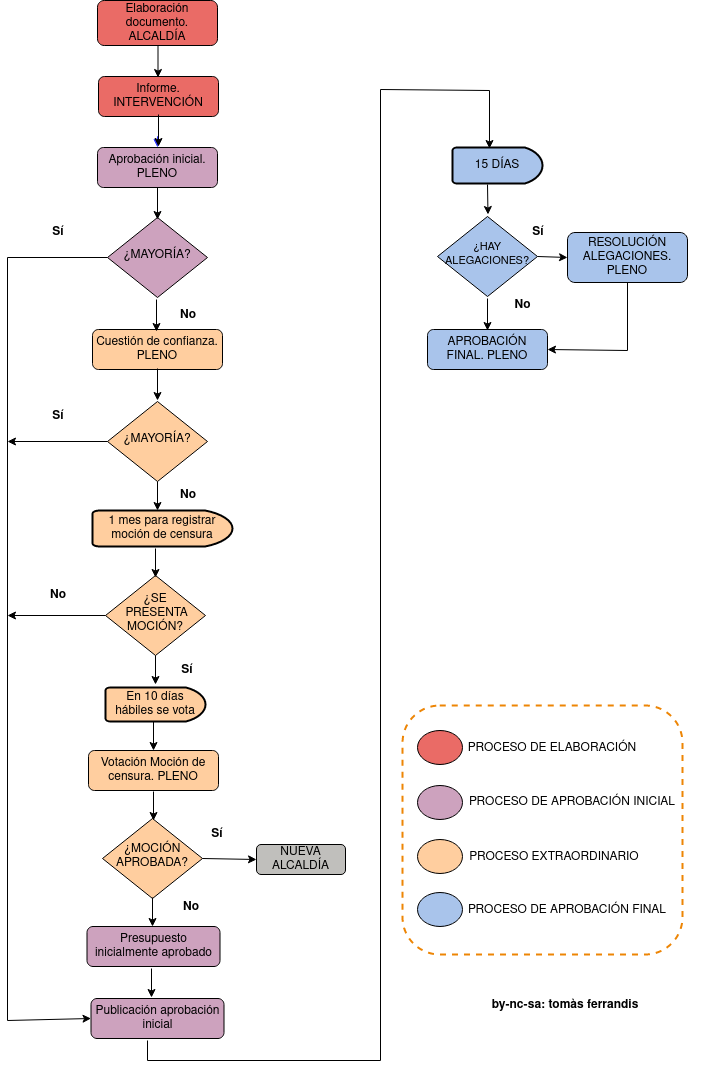
\includegraphics[width=5.90069in,height=9.10347in]{./png/aprovacionpresupuestolocal.png}

\hypertarget{fase-de-ejecuciuxf3n}{%
\subsection{FASE DE EJECUCIÓN}\label{fase-de-ejecuciuxf3n}}

Para el ejercicio del gobierno, los concejales delegados, dispondrán una
vez aprobado el presupuesto, de partidas habilitadas según sus
funciones. Ahora bien, esta potestad estará sujeta a unas normas
fundamentales incluidas en el documento único del presupuesto municipal:
las Bases de Ejecución.

\hypertarget{bases-de-ejecuciuxf3n}{%
\subsubsection{BASES DE EJECUCIÓN}\label{bases-de-ejecuciuxf3n}}

Se trata de un documento integrante del presupuesto donde encontraremos
detallados y adaptados a cada Entidad local, los procedimientos a seguir
para la gestión de su presupuesto general. Cada uno de estos
procedimientos explicado de forma precisa tras la consideración de
diversos artículos de dos o más normas con rango de ley. Esto nos da una
idea del sentido práctico de la Bases de Ejecución.

Las Bases de Ejecución adaptan a la realidad de cada municipio lo
dispuesto en la legislación, facilitando la comprensión y seguimiento de
los gestores municipales.

\hypertarget{modificaciones-del-presupuesto}{%
\subsubsection{MODIFICACIONES DEL
PRESUPUESTO}\label{modificaciones-del-presupuesto}}

La fase de ejecución implica la necesidad de ir ajustando las partidas
de ingresos y gastos según las necesidades, las circunstancias
cambiantes para que éste sea un instrumento contable eficaz.

\textbf{Vinculación jurídica}

Así pues, veremos la vinculación jurídica entre partidas que permite a
la Alcaldía realizar transferencias entre partidas sin necesidad de
hacer un expediente nuevo de modificación de créditos. Los créditos para
los gastos tendrán carácter limitador dentro de los niveles de
vinculación jurídica siguientes:

\begin{itemize}
\item
  Respecto de la clasificación por programas. Área de gastos.
\item
  Respecto de la clasificación económica: capítulo.
\end{itemize}

En lo referente a los créditos declarados en las mismas bases, la
vinculación jurídica se establece al mismo nivel de desagregación que se
observan en el presupuesto.

De tal forma que si hay dotación presupuestaria suficiente dentro de
este nivel de vinculación jurídica se podía realizar un gasto sin
dotación presupuestaria propia.

\textbf{Modificación de créditos}

Todo expediente de operación de crédito es iniciado por la Alcaldía,
desde la Intervención se informa tras el estudio de toda la información
detallada legalmente requerida. Dependiendo del tipo de operación, la
competencia para aprobarla es del propio Alcalde mediante resolución o
del pleno de la corporación mediante acuerdo plenario. Cuando sea el
pleno quien apruebe la concesión de créditos o suplemento, se procederá
como en la aprobación de los presupuestos en cuanto a publicidad y
trámite de alegaciones. A este respecto puede ser que el municipio
disponga de Ordenanza reguladora sobre Transparencia que obligue a la
publicación en el portal de la entidad de cualquier tipo de modificación
y, esta obligación, además se recoja en las bases.

Vemos como en la fase de aprobación de las modificaciones del
presupuesto, queda repartida entre el ejecutivo y el legislativo
dependiendo de la transcendencia para el equilibrio presupuestario que
tenga la operación.

Tipos de modificación de créditos:

\emph{Créditos extraordinarios y suplementos de créditos.} Cuando se
asigna más crédito a un gasto que debe realizarse dentro del ejercicio.
Se financia mediante:

\begin{itemize}
\item
  Remanente de tesorería. Incorporación del ejercicio anterior. Compete
  al Alcalde
\item
  Nuevos ingresos. Compete al Alcalde.
\item
  Anulación de créditos. Compete al Alcalde.
\item
  Operaciones de crédito a largo plazo. Solo si se destinan a
  inversiones o urgencias muy justificadas. Los tres primeros casos son
  competencia de la Alcaldía mientras que las operaciones de crédito son
  competencia del Pleno.
\end{itemize}

\emph{Transferencia de créditos.} Se trata de transferencias entre
partidas (no hay aumento del crédito total) de gasto que no tienen
vinculación jurídica. La aprobación es competencia del Pleno

\begin{itemize}
\tightlist
\item
  Incorporaciones de créditos. Reconocimiento demostrado de más derecho
  de los previstos. Compete al Alcalde.
\item
  Baja por anulación. Puede ser total o parcial y la aprobará el Pleno
\item
  Generaciones de crédito por ingresos. Competencias del Pleno.
\item
  Aportaciones de otras personas jurídicas.
\item
  Enajenaciones
\item
  Derivados de nuevas prestaciones de servicios
\item
  Incorporación de remanente de créditos
\end{itemize}

\textbf{Modificaciones del estado de ingresos}

Los tipos de modificaciones posibles son los que ya hemos tratado
anteriormente:

\begin{itemize}
\tightlist
\item
  Créditos extraordinarios y suplementos de crédito.
\item
  Operación de créditos
\end{itemize}

Los que no necesitan trámite de aprobación plenaria siendo competente el
Alcalde

\begin{itemize}
\tightlist
\item
  Nuevos o mayores ingresos a los previstos.
\item
  Incorporación del remanente de tesorería.
\end{itemize}

\hypertarget{la-pruxf3rroga}{%
\subsubsection{LA PRÓRROGA}\label{la-pruxf3rroga}}

Atendiendo a la legislación,\footnote{Art 169 TRLRHL y art. 21 del RD
  500/90.} si no se aprobase el presupuesto al inicio del ejercicio,
éste quedará automáticamente prorrogado. Este presupuesto prorrogado
contemplará como límite de créditos los iniciales en su momento de
aprobación un año antes. Es decir, no se incorporarán las modificaciones
presupuestarias que se aprobaron con la finalidad de atender necesidades
propias de programas y servicios del ejercicio cerrado. Sí que podrán
incorporarse los remanentes de ejercicios cerrados. En la propuesta se
detallarán todas las modificaciones para cumplir en lo indicado
anteriormente

En las Bases de Ejecución, además de recoger estas indicaciones legales,
podrán especificar un plazo para la presentación de la propuesta de
presupuesto prorrogado o indicar la Concejalía responsable.
Habitualmente se establece que la Concejalía Delegada de Hacienda haga
la propuesta antes del 15 de enero.

Si inicialmente no se ha cumplido el principio de especificidad
temporal, este no se abandona. Una vez aprobado el nuevo presupuesto,
éste tendrá como fecha de inicio el 1 de enero del año vigente y los
gastos e ingresos reflejados en el presupuesto prorrogado deberán
traspasarán al nuevo documento.

\hypertarget{el-proceso-de-gastos}{%
\subsection{EL PROCESO DE GASTOS}\label{el-proceso-de-gastos}}

La gestión del presupuesto de gastos se realizará mediante las fases que
se detallan:

\begin{itemize}
\tightlist
\item
  Autorización del gasto.
\item
  Disposición o compromiso del gasto.
\item
  Reconocimiento y liquidación de la obligación.
\item
  Ordenación del pago.
\end{itemize}

En este apartado haremos referencia a la Alcaldía o a la Presidencia de
la Entidad Local de forma genérica, aunque debemos entender que, en el
caso de un organismo autónomo, sería el órgano que según sus propios
Estatutos ostente la competencia concreta.

Todas las fases individualmente o agrupación de estas siguen el mismo
procedimiento:

1º PROVIDENCIA DE ALCALDÍA

2º INFORME DE INTERVENCIÓN

3º DECRETO DE ALCALDÍA O ACUERDO PLENARIO

\textbf{Autorización del gasto.}

El legislador ha aplicado un criterio similar al de las modificaciones
del presupuesto estableciendo un límite para el Alcalde o Alcaldesa que
podrá delegar en la Comisión de Gobierno o, en caso de no estar creada,
en alguna tenencia de Alcaldía. Estos límites serán los mismos que en la
aprobación de pliegos de contratación.:

\emph{Competencia de la Presidencia ( o quien ostente la delegación ).}

Inferiores al 10\% de los recursos ordinarios

\emph{Competencia del pleno}

Superiores al 10\% de los recursos ordinarios, plurianuales de más de
cuatro año o 6 millones de euros.

Así pues, el principio de división de competencias no consiste otorgar
toda la ejecución del presupuesto a la cámara (parlamentarismo), ni
tampoco al gobierno que sería el otro extremo de la tendencia iniciada
tras la II Guerra Mundial. Sino que se busca un equilibrio entre la
eficiencia y el control. No obstante, no debemos olvidar con la
periodicidad mínima establecida por la legislación local, la Alcaldía
debe dar cuenta en el primer pleno ordinario de sus resoluciones.

\textbf{Disposición del gasto.}

Corresponde al mismo órgano responsable de la autorización. En las Bases
pueden contemplarse la posibilidad de agruparse en la fase anterior para
ejecutarse en un mismo acto administrativo: autorización-disposición.

\emph{Acumulación de fases: AD}

En aquellos gastos en que la entidad conoce de antemano el importe
exacto y el nombre del perceptor, puede agruparse en un único Documento
contable ``AD''. Se trataría por ejemplo de adjudicaciones directas,
alquileres, importes anuales comprometidos, cuotas de amortización...

\textbf{Reconocimiento.}

Independientemente de qué órgano haya autorizado el gasto, el Pleno o el
Presidente, es este último el que tiene la competencia para el
reconocimiento y la liquidación de las obligaciones ya adquiridas.

La única excepción, lógicamente, es la que afecta a reconocimientos
extrajudiciales. Es decir, aquellos gastos que, a la hora de
contabilizarlos, se detecta que no existe dotación presupuestaria.

\textbf{Ordenación}

Es competencia del presidente de la entidad local. Éste podrá solicitar
al pleno la creación de una unidad de ordenación de pagos o de tesorería
en municipios de más de 500.000 habitantes que se encargará de esta
función.

Dependiendo de la existencia de alguna de estas unidades, las Bases
harán referencia a esta unidad, al Presidente de la entidad local u
órgano encargado en caso de organismo autónomo.

Plan de disposición de fondos. Marcará las prioridades en la ordenación
del pago. Lo encarga el responsable de ordenar los pagos y debe dar
prioridad a los pagos de personal y las obligaciones contraídas en
ejercicios anteriores sin olvidar la deuda pública.

\emph{Acumulación de fases: ADO}

En aquellos gastos donde legalmente obligatorio iniciar un expediente de
contratación, las tres fases se podrán acumular en un procedimiento
abreviado mediante el Documento contable ``ADO'' . Se trata de gastos de
reparación, mantenimiento, material de oficina, comunicaciones,
transportes, dietas y gastos de locomoción, gastos financieros o de
seguros y tributos\ldots{}

\textbf{Sobre los principios}

Como hemos podido deducir, el objetivo principal de las Bases de
Ejecución es flexibilizar dentro de la legislación los principios
económicos, contables y políticos los principios de especialidad
cualitativa, cuantitativa y temporal ( o los correspondientes principios
contables de especificación y ejercicio contable ), dotando de margen de
maniobra al gobierno local.

\hypertarget{fase-de-control}{%
\subsection{FASE DE CONTROL}\label{fase-de-control}}

El control en la ejecución del presupuesto se justifica por razones
financieras y políticas. Tal como ya hemos estudiado, se trata de
asegurar la correcta gestión de los fondos públicos desde la óptica
financiera y, por otra parte, del grado de cumplimiento del poder
ejecutivo -gobierno local -- en la gestión del presupuesto.

Así como la elaboración del presupuesto corresponde a la Alcaldía
(ejecutivo) mientras que a aprobación corresponde al pleno (legislativo)
en el control interviene el legislativo ( control interno) y, además del
poder externo, como mínimo, del Tribunal de Cuentas\footnote{LRHL Art.
  115. La fiscalización externa de las cuentas y de la gestión económica
  de las entidades locales corresponde al Tribunal de Cuentas.}.

\hypertarget{control-externo}{%
\subsubsection{CONTROL EXTERNO}\label{control-externo}}

\textbf{LOS ORGANISMOS DE CONTROL EXTERNOS (OCEX)}

Además del Tribunal de Cuentas contemplado en la Constitución y que
hemos estudiado en el tema habría que considerar otros organismos
autonómicos previstos en los Estatutos de Autonomía como es el caso de
la Sindicatura de Comptes en la Comunidad Valenciana.

El Síndicatura de Comptes es un ejemplo más de los Órganos de Control
Externo (OCEX). Se trata de organismos autonómicos que se encargan de la
fiscalización de las Entidades Locales en el ámbito autonómico además de
la misma Administración autonómica.

Ahora bien, debemos tener en cuenta que la Sindicatura de Comptes como
cualquier otro OCEX no tiene competencia para ejercer un enjuiciamiento
contable, aunque puede ejercer, solo por delegación del Tribunal de
Cuentas, alguna actuación.

La colaboración entre ambas instituciones, Tribunal de Cuentas y OCEX,
así como la publicación de datos correspondientes, entre otras, a las
Entidades que integran la Administración local. está contemplada y
regulada en la Ley de funcionamiento del Tribunal de Cuentas.

La mayoría de los OCEX están organizados a nivel europeo en la EURORAI
(Organización Europea de las Instituciones Regionales de Control Externo
del Sector Público) integrada por más de 70 organismos regionales de
Europa. A nivel de Estado forman parte todos de la ASOCEX ( Asociación
de Órganos de Control Externo ).

Ambas organizaciones persiguen la colaboración e intercambio de
información y experiencias.

\emph{Tabla 3 . OCEX y Tribunal de Cuentas}

\begin{longtable}[]{@{}
  >{\raggedright\arraybackslash}p{(\columnwidth - 4\tabcolsep) * \real{0.2400}}
  >{\raggedright\arraybackslash}p{(\columnwidth - 4\tabcolsep) * \real{0.3067}}
  >{\raggedright\arraybackslash}p{(\columnwidth - 4\tabcolsep) * \real{0.4267}}@{}}
\toprule\noalign{}
\endhead
\bottomrule\noalign{}
\endlastfoot
& \textbf{Funciones} & \textbf{Ámbito ( regulado )} \\
\textbf{Tribunal de Cuentas} & Fiscalización y enjuiciamiento & Estatal
( Constitución Española ) \\
\textbf{OCEX} & Fiscalización & Autonómico ( Estatuto de Autonomía ) \\
\end{longtable}

\hypertarget{control-interno}{%
\subsubsection{CONTROL INTERNO}\label{control-interno}}

El órgano de control interno en los municipios es la \textbf{Comisión
Especial de Cuentas} que está compuesta por concejales de todos los
grupos municipales. Su función principal es la de informar sobre las
cuentas anuales. Estas cuentas deberán hacerse públicas y presentarse
ante el pleno para que puedan ser aprobadas o rechazadas o formular en
su contra reclamaciones, reparos u observaciones. Evidentemente sin
perjuicio de que pueda denunciarse ante el Tribunal de Cuentas o
Sindicatura de Comptes cualquier irregularidad que entiendan en la
gestión económica o en las cuentas.

\textbf{Sobre los principios.}

El equilibrio de poderes que implica el principio de competencia queda
consagrado en esta fase. Por una parte, tenemos el del legislativo
entendido como los representantes de la voluntad popular en el Pleno o,
por extensión en la Comisión Especial de Cuentas para la fiscalización
interna de las cuentas. Por otra parte, el poder judicial y los demás
organismos de control externo.

El nuevo marco legislativo surgido a partir del la crisis de 2008 con el
objetivo de reducir la deuda pública y un mayor equilibrio
presupuestario, también incorpora nuevas medidas e instrumentos de
control en la gestión del presupuesto por parte del gobierno local.

\emph{Control externo:} Mecanismos que afectan directamente a la gestión
del gobierno local (autorizaciones para operaciones de crédito, remisión
de informes periódicos, obligaciones contra la deuda...)

\emph{Control interno}: Obligación de dar cuenta en sesión plenaria para
favorecer el control interno (cumplimiento de la regla de gasto o
período medio de pago a proveedores\ldots)

\emph{Control interno y externo:} solicitar aprobación plenaria (y dar
cuenta al Ministerio de Hacienda y Administraciones Públicas del plan
económico financiero o plan de ajustes)

\hypertarget{conclusiones}{%
\section{6. CONCLUSIONES}\label{conclusiones}}

\hypertarget{sobre-la-flexibilidad-en-la-gestiuxf3n}{%
\subsection{SOBRE LA FLEXIBILIDAD EN LA
GESTIÓN}\label{sobre-la-flexibilidad-en-la-gestiuxf3n}}

La flexibilización que de forma general se achaca al desarrollo del
Estado del Bienestar a partir de mediados del siglo XX tiene su versión
específica en el mundo municipal.

\textbf{Principios políticos}

Podríamos pensar que hay cierta relajación del \emph{principio de
competencia} al dotar a la Alcaldía de potestades en las diferentes
fases del presupuesto. La iniciativa en la elaboración, aunque sigue
siendo el Pleno quien lo aprueba, por ejemplo. Respecto al procedimiento
extraordinario de aprobación no puede ser entendida desde a óptica de
competencia como hemos aclarado anteriormente. En lo referente a la
ejecución vemos que la competencia queda repartida de forma racional y,
en el control interno, es el Pleno y la Comisión Especial de Cuentas la
que tienen toda la potestad.

Respecto al \emph{principio de universalidad}, la existencia de órganos
autónomos supone una relajación de este principio al saltarse la regla
de presupuesto único con la complejidad cada vez mayor de los organismos
autónomos.

El \emph{principio de claridad}, aunque la complejidad de la gestión
pueda ir en aumento, las nuevas tecnologías unidas a la, cada vez, mayor
exigencia en la transparencia contribuyen a mejorarlo.

La \emph{especificidad cualitativa, cuantitativa y temporal} no es fácil
de cumplir. Hemos visto como las Bases de Ejecución facilitan, dentro de
los límites legales, las transferencias entre partidas u otro tipo de
modificaciones en las previsiones iniciales.

Respecto al \emph{principio de publicidad}, éste, lejos de
flexibilizarse, cada vez está más presente en la gestión municipal y en
los cambios normativos que le afectan.

Además de la publicación de la obligación legal de publicar la
aprobación del presupuesto o las modificaciones que se hagan a efectos
de poder presentar alegaciones, la legislación estatal y la autonómica
en materia de transparencia \footnote{Art. 17 de la Ley 1/2022, de 13 de
  abril, de Transparencia y Buen Gobierno de la CV.}y buen gobierno
obligan a una publicidad activa de los presupuestos en páginas web y
portales de tal forma que hoy en día la ciudadanía tiene acceso a través
de internet a la información económica y presupuestaria de su municipio.

El concepto de gobierno abierto que promueve la legislación no se reduce
a la rendición de cuentas de la actividad pública, también incluye la
participación y colaboración ciudadana en las políticas públicas y la
propia gestión.\footnote{Art. 2.3 de la Ley 1/2022, de 13 de abril, de
  Transparencia y Buen Gobierno de la CV.}

\textbf{Principios contables.}

Los principios de \emph{presupuesto bruto} y el de \emph{especificación}
se han mantenido inalterables en el mundo municipal. En cambio, el
principio de \emph{unidad de caja} ha tenido que relajarse en la medida
que se han desarrollado organismos autónomos dependientes de la
Entidades Locales Por otra parte, el \emph{principio de ejercicio
cerrado} sabemos que no siempre se cumple y es una práctica habitual,
por citar un ejemplo, el reconocimiento extrajudicial de deudas del
ejercicio anterior al inicio del presente o la prórroga temporal del
presupuesto.

\textbf{Principios económicos.}

Estos son los principios que más han evolucionado en un sentido y, como
veremos en el siguiente apartado, posteriormente en el sentido
contrario.

La pérdida de sentido de la \emph{limitación del gasto} con la
implantación de Estado de Bienestar tuvo su versión en la Administración
Local con la ampliación de servicios más allá de los estrictamente
obligados por la legislación. Hablar de la \emph{gestión mínima} sería
hablar de un ``antiprograma electoral'', las promesas de los candidatos
y la valoración ciudadana de la gestión municipal
(\emph{accountability}) precisamente van el la línea contraria a la de
pedir una gestión mínima.

La \emph{neutralidad impositiva} entra en contradicción con el papel que
desde diferentes puntos de vista ideológicos se pretenda dar a la
gestión municipal. Pensemos por ejemplo en las privatizaciones de
servicios municipales o reversiones de éstos como el caso del servicio
de abastecimiento de agua potable que tratamos en el anterior trabajo.
Este principio representa una idea demasiado liberal que responde a la
falacia de querer ver al gestor público como el encargado de la
aplicación mecánica de reglas, carente de empatía social.

En lo que respecta al \emph{equilibrio contable} o la
\emph{autoliquidación de la deuda}, si bien venimos de una etapa de
relajación veremos en el siguiente apartado, como después de crisis de
2008 es un principio que ha creado cambiado las reglas de juego para la
gestión del presupuesto municipal mediante nuevas regulaciones y
modificaciones transversales de leyes existentes.

\hypertarget{sobre-la-vuelta-al-equilibrio-y-el-control}{%
\subsection{SOBRE LA VUELTA AL EQUILIBRIO Y EL
CONTROL}\label{sobre-la-vuelta-al-equilibrio-y-el-control}}

En el tema ya hemos abordado la nueva orientación dada referente a la
estabilidad presupuestaria. El nuevo marco normativo para los
ayuntamientos -a fecha de diciembre de 2022- en cuanto a medidas de
reducción de la deuda pública y equilibrio presupuestario quedaría
definido básicamente con la \emph{Ley Orgánica 6/2015,} la propia
\emph{Ley Orgánica 2/2012} modificada y algunas medidas respecto al
control interno y externo en la \emph{Ley 27/2013}.

A partir de esta legislación estatal, se imponen una serie de principios
y restricciones en la gestión presupuestaria entre los cuales
destacaremos los siguientes.

\textbf{Principio de estabilidad presupuestaria.} las corporaciones
locales deberán mantener una posición de equilibrio o superávit
estructural. La diferencia entre ingresos y gastos debe ser cero o
positiva. Esta diferencia indicará la capacidad de financiación.

\textbf{Principio de sostenibilidad financiera.} Se entenderá por
sostenibilidad financiera la capacidad para financiar compromisos de
gastos sin afectar al déficit, deuda pública y deuda comercial. El valor
que nos indicará la sostenibilidad será el Período Medio de Pago a
proveedores (PMP). Los ayuntamientos deberán mantenerlo inferior a 30
días y comunic al Estado mensualmente. En caso de que supere durante dos
meses seguidos este limite, se le impondrán al municipio medidas de
reducción de gastos, incremento de ingresos u otras de gestión de cobros
y pagos. Si la situación persiste, el Estado podrá retener su aportación
al ayuntamiento y pagar directamente a los proveedores.

\textbf{Regla del gasto.} El límite del gasto no financiero lo limitará
el Estado en función el Producto Interior Bruto (PIB). Este límite se
ajustará a las variaciones de la recaudación originados por cambios
normativos. En consonancia con el siguiente principio, los ingresos que
superen la previsión inicial se destinarán a reducir deuda pública.

\textbf{Prioridad en el pago del deuda pública.} Se dará prioridad al
pago de deuda pública e intereses. De forma coherente, no podrá aumentar
la deuda pública y cualquier operación de crédito deberá ser autorizada
por el Estado.

\textbf{Instrumentos y medidas de control y corrección.} Si los
ayuntamientos necesitan algún tipo de operación para obtener liquidez,
deben acordar con el Ministerio de Hacienda un \textbf{plan de ajuste}
coherente con el cumplimiento de los objetivos de estabilidad
presupuestaria y de deuda pública.

El incumplimiento del principio de estabilidad presupuestaria, del
objetivo de deuda pública o de la regla de gasto, obligará a la
corporación a presentar un \textbf{plan económico-financiero} para
reconducir la situación durante el ejercicio en curso y el siguiente. En
el plan deberá indicarse las causas del incumplimiento, los cambios
previstos con una descripción clara del temporalización y cuantificación
entre otros datos.

La aprobación de los planes económico-financieros como los planes de
ajustes es competencia del Pleno municipal.

\hypertarget{bibliografuxeda-y-otros-recursos}{%
\section{7. BIBLIOGRAFÍA Y OTROS
RECURSOS}\label{bibliografuxeda-y-otros-recursos}}

\begin{itemize}
\item
  Aragonés Beltrán, Emilio. 2011. ``Principio de suficiencia financiera:
  tasas locales''. Fundación Democracia y Gobierno Local, 2011-02.
\item
  Dalmau, Juan Carlos y Descalç, Asensi ( 2009). Una introdució a
  l'economía pública. València. Publicacions Universitat de València
  (PUV)
\item
  Ministerio de Hacienda y Función Pública
  \url{https://www.hacienda.gob.es/es-ES/Areas} Tematicas/Administracion
  Electronica/OVEELL/Paginas/ConsultaPTE.aspx
\item
  Tribunal de Cuentas \url{https://www.tcu.es}
\item
  Sindicatura de Comptes \url{https://www.sindicom.gva.es}
\end{itemize}

\hypertarget{legislaciuxf3n}{%
\section{8. LEGISLACIÓN}\label{legislaciuxf3n}}

\begin{itemize}
\item
  Constitución Española
\item
  Ley 1/2022, de 13 de abril, de Transparencia y Buen Gobierno de la
  Comunitat Valenciana
\item
  Ley 5/2021, de 5 de noviembre, reguladora del Fondo de Cooperación
  Municipal de los Municipios y Entidades Locales Menores de la
  Comunitat Valenciana
\item
  Ley 7/1985, de 2 de abril, Reguladora de las Bases del Régimen Local.
\item
  Ley 8/2010, de 23 de junio, de régimen local de la Comunitat
  Valenciana
\item
  Ley Orgánica 5/1982, de 1 de julio, de Estatuto de Autonomía de la
  Comunidad Valenciana
\item
  Real Decreto Legislativo 2/2004, de 5 de marzo, por el que se aprueba
  el texto refundido de la Ley Reguladora de las Haciendas Locales
\item
  Ley Orgánica 6/2015, de 12 de junio, de modificación de la Ley
  Orgánica 8/1980, de 22 de septiembre, de financiación de las
  Comunidades Autónomas y de la Ley Orgánica 2/2012, de 27 de abril, de
  Estabilidad Presupuestaria y Sostenibilidad Financiera.
\item
  Ley Orgánica 2/2012, de 27 de abril, de Estabilidad Presupuestaria y
  Sostenibilidad Financiera.
\item
  Ley 27/2013, de 27 de diciembre, de racionalización y sostenibilidad
  de la Administración Local
\end{itemize}

\end{document}
